% Chapter 2
% !TEX root = ../main.tex

\chapter{Techniques} % Main chapter title

\label{Chapter2} % For referencing the chapter elsewhere, use~\ref{Chapter1}

\lhead{Chapter 2. \emph{Techniques}} % This is for the header on each
%page -
%perhaps a shortened title

%----------------------------------------------------------------------------------------

% Section Signal Pre-processing
% !TEX root = ../../main.tex

\section{Signal pro-processing and sensor fusion for timed patterns}
  Describe how data is collected and processed, the form of the data (continuous to discrete, amplitude, energy, frequencies, etc).
  Include feature extraction, like PCA, FFT, energy, mean, but discuss it further in subsection.
  Only the concepts will be explained and the scheme of the computations (or simply formulas), no precise implementations.
  Mention only shortly with meaning, no further explanation.

  --------


    \subsection{Signal fusion}
    Signal fusion is a broad field of research and application and many different interpretations exist.
    The function and interpretation used in this thesis follows the definition from \cite{elmenreich2001introduction}, stating:
    \begin{center}
      \textbf{Sensor fusion} is the combining of sensory data or data derived from sensory data such that the resulting information is in some sense better than would be possible when these sources were used individually.
    \end{center}
    This can essentialy be considered as a form of synergy, in which the combination of the sensors provide more information than the sum of the raw output.
    For the application of this thesis we will focus on direct fusion of raw data, which can be applied to both homogeneous and heterogeneous sensors.
    The fusion stage will combine the data into a single representation, which can be interpreted by the controlling system.
    This differs from mere multisensor integration, in which the controlling system is responsible for processing and interpreting the data from different sources.
    Figure \ref{fig:sensor_fusion} shows the difference.

    \begin{figure}[htbp]
      \centering
        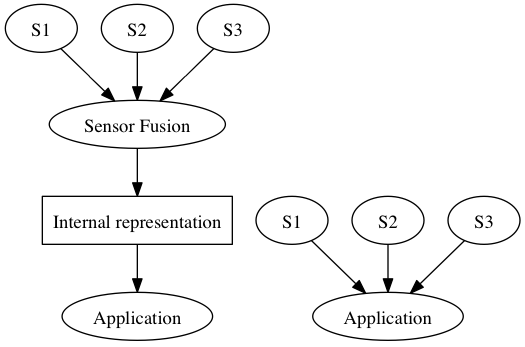
\includegraphics{./Figures/graphs/sensor_fusion.png}
        % \rule{35em}{0.5pt}
      \caption[K-means]{On the left \emph{Sensor Fusion} and on the right \emph{Multisensor integration}}
      \label{fig:sensor_fusion}
    \end{figure}

    Using the single representation, the computational and system complexity can be reduced.
    The representation forms a standardized and normalized interface from the sensors to the system, which create independence and modularity of sensors.
    Other benefits as a result from sensor fusion include \cite{elmenreich2001introduction}:
    \begin{itemize}
      \item \textbf{Robustness en reliability:} When the system incorporates multiple sensors as redundancy, the system becomes more stable in case of partial failure.
      \item \textbf{Extended spatial and temporal coverage:} With multiple sensors a broader spectrum can be analyzed, both in the case of homogeneous and heterogeneous combinations.
      \item \textbf{Increases precision:} Sensors typically have a range and domain of measurements.
      By combining a set of heterogeneous sensors, the overall range of observervation is increased.
      \item \textbf{Reduced ambiguity and uncertainty:} In case of high uncertainty about a observation, the observation of other sensors can confirm it.
    \end{itemize}

    Sensor fusion can be applied on multiple levels. A rough diversion over three levels is:
    \begin{itemize}
      \item \textbf{Low-level:} Raw sensor data is combined which is considered to be more informative than the original sources.
      \item \textbf{Intermediate-level:} Also known as \emph{feature fusion} combines the features which can be extracted from the data.
      See also section \ref{sec:feature_extraction}.
      This data would be applicable to segmentation **[???].
      \item \textbf{High-level:} Fusion of this level will support decision making, optionally followed by actions taken by the system to the environment or conclusion being drawn from the environment.
    \end{itemize}


    \subsection{Signal smoothing}
    What, why and how.

    \subsection{Feature extraction}
    \label{sec:feature_extraction}
    What, why and how.

\section{Temporal Segmentation}
This section will give an introduction and in-depth analysis of temporal segmentation.

\subsection{Aims of segmentation}
When processing and analyzing time series of data, e.g. motion measurements, stock market fluctuations or natural language, first a low-level division between the discriminative parts of the stream must be made.
One can view this as splitting the series into the \emph{atoms}, which are the building blocks of the total stream.
These building blocks will be the aggregation of non-overlapping, internally homogeneous segments \cite{himberg2001time}.
This means that the data points inside a segment should have some resemblance relation to each other and their difference lies between some boundary.
The process of segmenting can be viewed as a subproblem to context analysis of time series.
Temporal segmentation is closely related to temporal clustering, although it is a stricter, and simpler, process.
Whereby clustering only restricts the data points on their distance relation (as used in a Voronoi diagram), within a segment the data points must also be contiguous.

The task of segmentation can be performed in a manual matter, by cutting and labeling parts of the stream into coherent parts.
This would require human (expert) knowledge and does not yield a clear cut because of ambiguity.
With increasing storage abilities and easier motion capture systems, there is a desire for automated systems which perform the segmentation task unsupervised.
Some algorithms used have the (often desired) side-effect of also clustering the segments, such that classes of segments can be discovered in the time series.
These algorithms would not only be able to make a distinction between walking, sitting and walking, but would also recognize the reappearance of the walking activity.

\subsection{Formal definition}
Formally, temporal segmentation is dividing a time series $s$, which consists of $N$ samples $\mathbf{x}(1),\mathbf{x}(2),\dots,\mathbf{x}(N)$ from $\mathbf{R}^d$.
Individual \emph{segments} are referenced by $s(a,b)$, consisting of the consecutive samples $\mathbf{x}(a),\mathbf{x}(a+1),\dots,\mathbf{x}(b)$, $a \le b$.
Let $s_1 = s(a,b)$ and $s_2 = s(b+1,c)$ be two segments, then their concatenation is $s_1s_2 = s(a,c)$.
A segmentation $S$ of $s$ consists of a sequence of $k$ non-empty segments $s_1s_2 \dots s_k = s$.
This notation is adopted from \cite{himberg2001time}.

As stated, informally each segment should be internally homogeneous.
This can formally be measured with an cost function $F$, indication the heterogeneity of a segment.
The overall aim is to minimize the cost $F$. The cost of a segment is a function from the data points and the number of data points
$n = b - a + 1$ and is expressed as
\begin{equation}
	\label{eq:segment_cost}
	\mathrm{cost}_F (s(a,b)) = F(\mathbf{x};n|\mathbf{x} \in s(a,b))
\end{equation}
The cost of a \emph{k-segmentation} $S$ is the summation of the costs of the $k$ segments:
\begin{equation}
	\label{eq:segmentation_cost}
	\mathrm{Cost}_F (s_1 s_2 \dots s_k) = \sum_{i=1}^{k} \mathrm{cost}_F (s_k)
\end{equation}
With the objective of minimizing the cost function, the optimal $k$-segmentation $S_F^\mathit{opt}(s;k)$ is the segmentation with minimal $\mathrm{Cost}_F(s_1 s_2 \dots s_k)$ over all possible $k$-segmentations.

The cost function, to calculate the heterogeneity of a (set of) segment(s), can be any function.
A simple and natural function would be the sum of variances of the segments.
The overall cost function would then be
\begin{equation}
	\label{eq:cost_variances}
	\mathrm{Cost}_V = \frac{1}{N} \sum_{i=i}^{k} \sum_{j=c_{i-1}+1}^{c_i} \|
	\mathbf{x}(j) - \mu_i \|^2
\end{equation}
where $\mu_i$ is the mean vector of data points in segment $s_i$.

\subsection{Application in research fields}

[CHARACTERISTICS OF HUMAN MOTION]
temporal variability, invariance over time, metrics over actions.

[COMPUTER VISION]

[GRAPHICS/VIDEO]

[DATA-MINING]

[MODEL BASED]

To analyze time series it is often preferred to divide the stream in segments of correlated data.
After dividing, each segment represent a period in time in which the same activity is performed.
Or, stated otherwise, it results in transitions moments between activities.

\subsection{PCA Based Methods}

Many fields of research have been active in the unsupervised segmentation of data.
Many authors rely on a form of Principal Component Analysis (PCA), as used a.o. in \cite{barbivc2004segmenting}.
Often PCA is used to reduce the dimensionality of the data being processed [REFERENCE] by only using the top $r$ dimensions to describe the data set.
It is observed that data series of simple motions have a lower dimensionality then complexer motions.
When a simple (repetitive) motion is about to end and fluently transforms in a new motion, there will be a window of time in which a high dimensionality will be present, due to the new motion.
After this period of transition, the dimensionality will decrease, since only the new simple motion is present in the window of time.
The first algorithm of \cite{barbivc2004segmenting} is based on this principle.

Given a set of data points, a lower dimensional hyperplane can by constructed to which the data points can be projected.
This projection on a lower dimension introduces a error to the original position.
When the error is fixed, less dimensions are needed for simple motions in which movements of body parts are highly correlated.
For segments in which the data points are lesser correlated, e.g. because of transition state, a higher degree of dimensions of the hyperplane is needed to represent the data with equal error degree.
When the dimensionality is reduced from $d$ to $r \le d$, the ratio of error $E_r$ can be calculated as
\begin{equation}
	E_r = \frac{\sum_{j=1}^{r} \sigma_j^2}{\sum_{j=1}^{d} \sigma_j^2}
\end{equation}

where $\sigma_j$ are the singular values as a result from Singular Value Decomposition (SVD), which is closely related to PCA \cite{shlens2005tutorial}.

In \cite{barbivc2004segmenting} the stream of frames is analyzed on cut-frames to find transitions between action.
First, for a number of $k$ frames (e.g. the equivalent of 2.5 seconds) the required dimensionality $r$ to keep the error $E_r$ below some threshold $\tau$ is calculated.
This will yield in an error $e_i$ for the first $i$ frames.
When more frames are added to the window, the error will increase with a low constant when it is still in the same activity, due to noise in the activity.
When a new activity starts, e.g. at frame $j$, the error at frame $j$ will start increasing faster.
This can be expressed by the derivative of the error rate $d_i = e_i - e_{i-l}$, where $l$ is a constant to remove noise.
From this derivative the mean and standard deviation can be calculated, for each point.
When a derivative $d_j$ rises more than a factor $k_\sigma = 3$ standard deviations from the mean, a transition point is encountered.
The previous frames are then cut from the sequence (as a segment) and the algorithm starts over.

*** [figure to illustrate derivative and standard deviation]

A second approach in \cite{barbivc2004segmenting} uses the probabilistic variant of PCA (PPCA) to model the data set as a Gaussian distribution instead of ignoring the frames which do not fit in the subspace.
Over windows of frames the mean and variance are calculated.
In a forward manner the Mahalanobis distance of a new window of frames is calculated, which represents the likelihood of the new window belonging to the same segment as the original widow.
When the distance decreases, the likelihood increases which happens when the motions in the becomes more homogeneous.
When a peak in the distance is reached, the new window of frames indicates a heterogeneous collection of motions in the window and thus a low likelihood of membership and a indication of a transition.
In order to distinct activities and sub-activities (which require a subset of motions is a distinct activity) the algorithm is also processed backward over the data series.

*** [figure to illustrate mahalanobis distance measure and peaks]

The third algorithm in \cite{barbivc2004segmenting} is based on the observation that data points (frames) tend to form clusters in the space.
These clusters are represented by $k$ Gaussian distributions for which each the Expectation-Maximization (EM) algorithm estimates the mean $m_j$, covariance matrix $\sum_{j}$ and prior $\pi_j$.
With all the Gaussian distributions estimated, the data points are assigned to the cluster with the highest membership likelihood.
When two consecutive frames $x_i$ and $x_{i+1}$ belong to different clusters, a transition of activities is recognized.
Note that this algorithm succeeds in segmenting the data and also labels the similar simple activities.

A drawback in this system, and many others which implement a variant of the $k$-means algorithm, is that the number of clusters $k$ need to be predetermined.
To cope with this, often the algorithm is performed multiple times for different values of $k$.
Using some criteria, e.g. the Bayesian Information Criterion \cite{pelleg2000x} or the Davies-Bouldin Index which guides $k$-means clustering as used in \cite{krause2003unsupervised}.

\subsection{Statistical methods}
An method to process data, or create a basis for further processing, is by analyzing the statistical properties of a data set.
When there is a continuous stream of data, it is possible to extract events by comparing the statistical properties of sliding time windows.
By definition, events have a different statistical profile then their background.
When two consecutive actions are regarded as the background, then a transition is an event between them.

In \cite{guenterberg2009automatic} a automatic system is used to segment a continuous stream of data.
By calculating features as activity level from the standard deviation of a sliding window and applying Adaptive Thresholds, the data can be segmented in active and rest parts.
There is no model representation.

\subsection{Hidden Markov Models Based Methods}

\subsection{Bayesian Methods}

\subsection{Principal Component Analysis}
When working with simple 2- or 3-dimensional data it is often, for humans, easy to discover patterns in the set.
The data can be plotted and the lines or planes among which the data points lie gives an indication of the pattern.
With Principal Component Analysis (PCA) this process is also possible for automated systems.
With this method the overall form of a set of data points can be represented, the most discriminative dimensions can be found, the dimensionality of a set can be reduced (which yield in data compression) or the result can be used to characterize and differentiate sets of data points.

The following steps are performed, which are explained below and illustrated in figure *** [add figure with plot of sets]:

\begin{enumerate}
	\item \textbf{Gather data} and represent them in a chosen number of features,
	\item \textbf{Subtract mean} to center the data around the axis. The new data set will have mean zero,
	\item \textbf{Generate covariance matrix} by calculating all pairwise feature variances,
	\item \textbf{Calculate Eigenvectors and Eigenvalues} of the covariance matrix.
	The Eigenvectors are then normalized to make further calculations easier,
	\item \textbf{Generate feature vector} which indicated which features are characteristic or meant to keep in de data set, by comparing the Eigenvalues.
\end{enumerate}

The workings of the PCA \cite{smith2002tutorial} relies on the concepts of standard deviation, variance, covariance, eigenvectors and eigenvalues of matrices.
These concepts will be discussed very briefly \footnote{For a more in-depth discussion we would like to refer the reader to \cite{jolliffe2005principal}}.
The standard deviation and variance of a set are measures for the spread around the mean for a single dimension, or feature.
The covariance between two features (dimensions of the data points) indicates how they are related; when positive the two features will increase together; when negative one will decrease when the other increases and when zero they are unrelated.
The covariance matrix gives all the covariances for all pairs of features.
This matrix is symmetrical about the diagonal and the values on the diagonal are the variances for each feature.
For this matrix the eigenvectors can be computed. Eigenvectors have the characteristic that when they multiply a matrix, the resulting vector is a multiple of the Eigenvector.
The amount by which it is the multiple is the Eigenvalue.
This is illustrated in formulae~\ref{eq:no-eigenvector} and \ref{eq:eigenvector}.
The second formula shows an Eigenvector $ \left( \begin{smallmatrix} 3 \\ 2 \end{smallmatrix} \right)$ and its associated Eigenvalue, 4.
The vector in the first formula is not an Eigenvector.

\begin{equation}
	\label{eq:no-eigenvector}
	\begin{pmatrix} 2 & 3 \\ 2 & 1 \end{pmatrix}
	\times
	\begin{pmatrix} 1 \\ 3 \end{pmatrix}
	=
	\begin{pmatrix} 2 \cdot 1 + 3 \cdot 3 \\ 2 \cdot 1 + 1 \cdot 3
	\end{pmatrix}
	=
	\begin{pmatrix} 11 \\ 5 \end{pmatrix}
\end{equation}

\begin{equation}
	\label{eq:eigenvector}
	\begin{pmatrix} 2 & 3 \\ 2 & 1 \end{pmatrix}
	\times
	\begin{pmatrix} 3 \\ 2 \end{pmatrix}
	=
	\begin{pmatrix} 2 \cdot 3 + 3 \cdot 2 \\ 2 \cdot 3 + 1 \cdot 2
	\end{pmatrix}
	=
	\begin{pmatrix} 12 \\ 8 \end{pmatrix}
	=
	4 \times \begin{pmatrix} 3 \\ 2 \end{pmatrix}
\end{equation}

 It are these Eigenvectors and Eigenvalues that makes PCA possible.
 Given a matrix of size $n \times n$ (only square matrices have Eigenvectors), $n$ Eigenvectors can be found.
 Each Eigenvector is perpendicular, or orthogonal, to the others.
 The Eigenvectors combined describes the lines over which the data is plotted.
 The Eigenvector with the largest Eigenvalue is the \emph{principal} component of the data set.
 It is said that it is the most significant feature.
 Thus the Eigenvectors, and thereby the features or dimensions of the data set, can be sorted on significance by the Eigenvalues.

With this ordering there are a few applications possible.
The first is to just make a (comprehensible) representation of the data.
The Eigenvectors describe the cloud of data points and thus are a compressed representation of the data.
When the original data points are to be compressed, it is possible to remove the least significant features and reconstruct the data points from the resulting Eigenvectors.
This will yield in a lossy compression. *** [figure to illustrate].
An extension of this application is to determine the number of features needed to keep the compression within a certain error criterion, as used in \cite{barbivc2004segmenting}.
Sets of data can then be distinguished by the number of features needed to describe the points.

*** [graph, a bit of formulae with sets and dimensions]


%-------------------


\subsection{Hidden Markov Models}
Many dynamic systems can be viewed as some sequence of consecutive states which are observable by the world.
These kind of systems are known as Markov Chains.
When the state in which the system is can not be observed with complete certainty, a system known as a Hidden Markov Model (HMM) can be constructed.
It has been shown that HMMs are effective on in the task of speech recognition \cite{rabiner1989tutorial}.
Because of some resemblance between natural speech construction and human activities, modifications have been able to classify human activities \cite{guenterberg2009distributed} and extensions are implemented which create layers of HMMs to handle different granularity over time and reduce retraining \cite{oliver2002layered,perdikis2008recognition}.
A HMM is a state-space model representing a single model for each label which needs to be classified.

Formally, a Hidden Markov Model is characterized by the following elements
\cite{rabiner1989tutorial}:
\begin{enumerate}
	\item
		A number of $N$ states in the model.
		These states are a representation of the underlying mechanism of the system and can not be directly observed from outside (hence the \emph{hidden} model).
		Individual states are referenced by $S = \{S_1, S_2, \dots, S_N \}$ and a single state in time $t$ is denoted by $q_t$.
	\item
		An alphabet of $M$ discrete observable symbols for each state.
		An observed symbol is the only indication of the systems current situation.
		Each individual symbol is referenced by $V = \{ v_1, v_2, \dots, v_m \}$.
	\item
		A state transition probability distribution $A = \{ a_{ij} \}$ indication the probability of being in state $j$ at time $t+1$ when the state on time $t$ was $i$:
		\begin{eqnarray}
			a_{ij} = P [ q_{t+1} = S_j | q_t = S_i ], & 1 \le i, j \le N
		\end{eqnarray}
		Note that by setting the probability $a_{ij}=0$ for some $i$ and $j$ indicates that $j$ is not reachable from state $i$.
	\item
		A symbol observation probability distribution in state $j$, $B = \{b_j(k) \}$, where
		\begin{eqnarray}
			b_j(k) = P[ v_k\ \mathrm{at} \ t | q_t = S_j], & 1 \le j \le N \nonumber \\
			& 1 \le k \le M
		\end{eqnarray}
		Note that every symbol can be observed in every state.
	\item
	The initial state distribution in which the system starts $\pi= \{ \pi_i \}$ where
	\begin{eqnarray}
		\pi_i = P[q_1 = S_i], & 1 \le i \le N
	\end{eqnarray}
\end{enumerate}

This system is often abbreviated to
\begin{equation}
	\lambda = \{ \pi_i, a_{ij}, b_j(k)\}
\end{equation}
The HMM will act as a generator giving a sequence of $T$ observations, each being a symbol from $V$:
\begin{equation}
	O = O_1, O_2 \dots O_T
\end{equation}

Given the characteristics of a specific HMM, there are three major application which serve the classification of an activity.
The first application is, given a sequence of observations $O = O_1,O_2,\dots,O_T$, to label this sequence with the activity with the highest associated probability for that label, e.g. compute $P(O|\lambda)$ for each model $\lambda$.
The second task a HMM can perform is to \emph{explain} a observation sequence $O$, by choosing an optimal corresponding state sequence $Q = q_1,q_2,\dots,q_T$.
The last application is more of a problem statement, being the task to train the HMM to adjust the parameters $\lambda = \{ \pi_i, a_{ij}, b_j(k)\}$ to maximize $P(O|\lambda)$.
In the overall task of activity recognition, one would first use the last application to train a set of HMMs with the provided and labeled training data.
The second application can be used to further optimize the HMM (set the number of states, adjust vector codebook etc.) and improve the capability of modeling the activities.
Finally, when the system is provided with unlabeled data the first application is used to identify the observed sequence with trained examples, by comparing the probability result of multiple HMMs.

Generally a HMM can be fully connected, or ergodic model.
Other configurations are also possible, of which the left-right model, or Bakis model, is popular for temporal applications \cite{rabiner1989tutorial}.
This because the structure of the state probability distribution resembles the construction of possible states over time.
This left-right model can be generalized by setting
\begin{eqnarray}
	a_{ij} = 0, & j > i + \Delta
\end{eqnarray}
for some $\Delta$, indicating the possible \emph{distance} of the jumps over states.

*** [INSERT GRAPHICS SHOWING STRUCTURE OF HMM]

*** [discrete and continuous HHMs]

*** Applications of HHM: \cite{shi2009towards} uses 10 coefficients extracted with FFT from 6 axis (3 times accelerometer and 3 times gyroscope).
Example of continuous HMM (?).
Recognition rates fo 50\%-100\%.

In \cite{oliver2002layered} it is stated that HMMs are robust mechanisms with respect to changes in temporal segmentation of observations, although they suffer from a few problems when applied to reason about longer and complexer sequences over time.
They state that, especially with limited training data, the HMM tend to be overfitted and tend to lack structure and have an excess of parameters.
The overcome this limitation, they introduce a Layered Hidden Markov Model (LHHM) which they show is more robust to temporal changes in observations.
They make use of the hypothesis from the field of psychology, that human behavior is hierarchically structured \cite{zacks2001event}.
In \cite{perdikis2008recognition} a layered construction of HMMs is used which feeds the low-level data from a sliding window to the lower layer.
This layer will recognize simple motions, such as moving the arm in a pre-defined segment.
The results from these lower HMMs are then fed to a higher-level layer of HMMs which are able to recognize abstract motions, such as adjusting a monitor and picking up a pen.
The results showed that the layered system was better at recognition then a similar single-layered setup.
It was also robust in the sense that when the environment was changed, only the relatively simple low-level HMMs needed to be retrained.

*** [DIAGRAM WITH EXAMPLE OF LOW- AND HIGH-LEVEL HMMs, SUCH AS MOVING ARM, PICKING UP PEN]


*** Viterbi algorithm / path; find the most likely sequence of cause-states for the observed measures.


%-------------------



\subsection{Segmentation as clustering}
In the previous section the discussed methods all relied on the stream of data points and tried to find cuts the discriminate between successive different type of activities.
An other approach is to consider the tasks of segmentation as a type of clustering \cite{zhou2008aligned}.
In clustering the objective is to assign labels, or classes, to all the data points indication a similar type of activity.
A clustering $\mathcal{L}$ is thereby more informative then a segmentation but is also harder to produce.

A clustering $\mathcal{L}$ is generated from a sequence of elements $\mathbf{X}$ which is decomposed in $m$ disjoint segments, each belonging to one of the $k$ classes.
A segment $\mathbf{Y}_i \hat{=} \mathbf{X}_{[s_i,s_{i+1})}$ is composed of frames from position $s_i$ to $s_{i+1}$.
A vector $g_{ci} = 1$ indicates class membership if $\mathbf{Y}_i$ belongs to class $c$, otherwise $g_{ci} = 0$.

When regarding segmentation of human motion as a task of clustering the difficulty is to model the temporal variability of actions and defining a robust metric between temporal actions.
To overcome this, \cite{zhou2008aligned} introduces Aligned Cluster Analysis (ACA), by minimizing
\begin{equation}
	\label{eq:ACA}
	J_{\mathit{ACA}}(\mathbf{G},\mathbf{s}) = \sum_{c=i}^{K} \sum_{i=1}^{m} g_{ci} \mathit{dist}_c (\mathbf{X}_{[s_i,s_{i+1})})
\end{equation}

The characteristic of ACA is that is enables segments to span over different number of data points, whereas the standard kernel $k$-means algorithm results in equally sized segments.
[!!! TRUE?!] The second difference is that the kernel used in $\mathit{dist}_c$ to measure the distance from a segment to the class which it is assigned to uses the Dynamic Time Alignment Kernel [REFERENCE?] to measure between time series.

%----------------------------------------------------------------------------------------

\section{Clustering}

This section will give an introduction and overview to clustering of data.
When processing time series of data the line of distinction between segmentation and clustering is very fine.
This section will introduce clustering for the purpose as used in this project.

Data clustering can be used with two different applications, exploratory or confirmatory \cite{jain1999data}.
In the former, the purpose is to discover clusters in a point cloud of data points.
Here the cluster is defined as a group of homogeneous data points measured by some coherence measure, often a distance function with the data points being defined as vectors.
The produced clusters, which together form a representation of the data examined, can be used in the latter application to assign new provided data points to a cluster and thereby classify them.

Depended on the precise setup, clustering can be used as a successive step after or an implementation of temporal segmentation.
When temporal segmentation is used to create successive coherent data points, clustering can be used to recognize the same activities in different points of time.
The data points provided to the clustering will be some representation of each segment and each segment will be labeled with a activity.
Another mechanism could be to extract features from the raw data points and use these to create clusters directly *** [temporal modifications].
Both mechanisms requires the exploratory and confirmatory phases.

The exploratory phase roughly consists of the following five steps
\cite{jain1999data}
\begin{enumerate}
	\item data point representation,
	\item definition of coherence,
	\item grouping data points,
	\item cluster abstraction,
	\item output qualification
\end{enumerate}

The first step is to find a \emph{representation} of the data points and clusters, considering the number, type and scale of the features and the number of desired classes to cluster in.
When dealing with high-dimensional data points a \emph{feature selection} can be performed to use only the most discriminating features.
When the raw features are not useful enough, \emph{extraction} can be used to create new synthetic features. *** [qualitative versus quantitative/conceptual]

When the data points are represented in a meaningful way, the measure of \emph{coherence} between pairs of points must be defined.
Often this is implemented as the Euclidean or Mahalanobis distance when the data points are represented as vectors or other similarity measures for conceptual patterns.

In the most critical step, the \emph{grouping}, the data points with the highest coherence are linked together to form a cluster.
The result can be a hard partition over the data or a fuzzy membership degree to each cluster for each data point.
When applying rules for merging and splitting cluster, a hierarchical partition is constructed.
Partitional clustering algorithms assign data points to clusters by optimizing some criterion, e.g. the mean squared distance from each data point to the clusters' centroid.

Especially in case of large data sets, the resulting clusters will be defined by many data points.
To form a compacter and simpler representation, \emph{abstraction} can be used.
This will simply analysis by humans or automated systems.
A common abstraction is to use the clusters' centroid \cite{diday1976clustering} or parameters of Gaussian patterns.

The final step which can be applied to the resulting partition is some \emph{qualification}.
The quality of multiple partitions can be compared and the validity of the partition can be determined.
A partition is valid if reasonably it could not been constructed by change or as some random process.
External references of models can be used to compare, or the internal data points can be examined. *** [better wordings]


%-------------------

\subsection{Formal definition}





%-------------------

\subsection{Application is research fields}


%----------------------------------------------------------------------------------------

\section{Temporal pattern recognition}

\subsection{Dynamic Time Warping}
Used to measure similarity between time sequences.
Exact matching is high-cost, so approximations such as Minimum Bounding Rectangles are used.

\subsection{k-means clustering}
[EXPLAIN] divide data set $n$ into $k$ clusters. Follows the outline in figure~\ref{fig:k_means}

Among many unsupervised clustering techniques, $k$-means is successfully applied to large data sets.
It is simple to implement and linear in time complexity so computationally attractive \cite{jain1999data}.
A drawback of the method is that the results of the algorithm greatly depends on the initial configuration (the data points which will act as centroids) and the number of cluster $k$ must be determined beforehand.

\begin{figure}[htbp]
	\centering
		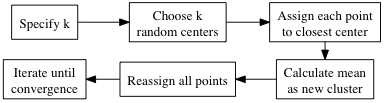
\includegraphics{./Figures/k_means.png}
		\rule{35em}{0.5pt}
	\caption[K-means]{Outline of the $k$-means algorithm.}
	\label{fig:k_means}
\end{figure}

Generally, the $k$-means methods will minimize the squared error for a clustering $\mathcal{L}$ criterion which is defined as the distance from thedata points the centroid for each cluster in $\mathcal{K}$.
This is expressed as optimizing to a local optimum the energy function
\begin{equation}
	\label{eq:k-means energy}
	e^2(\mathcal{K},\mathcal{L}) =
	\sum_{j=i}^{K}\sum_{i=1}^{n_j}\|\mathbf{x}_i^{(j)} -
	\mathbf{c}_j\|^2
\end{equation}

There are several limitation on the $k$-means method.
One of these is that only spherical shapes of cluster can be generated.
One of the extensions is kernel $k$-means \cite{scholkopf1998nonlinear}, which implicitly projects the data points to a higher dimension and thereby is able to form irregular shaped cluster.

\subsection{Self-organizing Map}

\subsection{Support Vector Machine}

\subsection{Na\"{i}ve Bayes}

\section{Unsupervised clustering of temporal patterns}